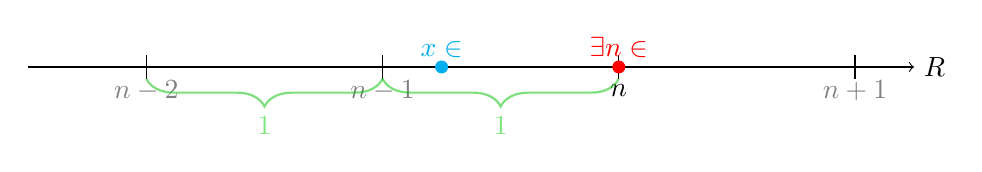
\begin{tikzpicture}[scale=1.5]
	% Draw the number line
	\draw[->] (-1, 0) -- (6.5, 0) node[right] {$\mathbb{R}$};
	
	% Mark points on the number line
	\foreach \x in {0, 2, ..., 6}
	\draw (\x,0.1) -- (\x,-0.1);
	
	% Mark point x
	\filldraw[cyan] (2.5, 0) circle (0.05) node[above] {$x\in\R$};
	
	% Mark point n
	\filldraw[red] (4, 0) circle (0.05) node[above] {$\exists n\in\N$};
	
	\node[gray] at (6,-0.2) {$n+1$};
	\node[] at (4,-0.2) {$n$};
	\node[gray] at (2,-0.2) {$n-1$};
	\node[gray] at (0,-0.2) {$n-2$};
	
	\draw[decorate, decoration={brace, amplitude=10pt}, thick, color=green!75!black, opacity=.5] (4, -0.1) -- (2, -0.1) 
	node[midway, below=10pt, color=green!80!black] {\( 1 \)};	
	\draw[decorate, decoration={brace, amplitude=10pt}, thick, color=green!75!black, opacity=.5] (2, -0.1) -- (0, -0.1) 
	node[midway, below=10pt, color=green!80!black] {\( 1 \)};	
\end{tikzpicture}